\scalebox{0.8}{\textit{Reference: \cite{lubanovic2019introducing} Chapter 11}}

A \emph{module} is a file that contains Python code. Large programs are more manageable when divided into modules. Many functions in the standard Python library are stored in modules. The \code{math} and \code{random} modules are common examples. These shouldn't require additional installation to use if you've downloaded Anaconda. 

To use a module, you must import the module with an import statement, \code{import math} for example. Then any function in that module can be accessed by using the function name, prefixed by the module name and a dot. To use \code{sqrt} from \code{math}, you must use \code{math.sqrt(81)}. 

You can import just a specific function with syntax like the following: \code{from math import sqrt}. Then \code{sqrt} can be accessed without the \code{math.} prefix. Running \code{from math import *} is called a wildcard import and will import every function in the module. 

Finally, you can \emph{alias} a specific module, library, or function with an \code{as} clause. There are conventional aliases for many modules. Pandas, NumPy, and Datetime are libraries we will cover later. These are typically imported with aliasing as in the below. 

\begin{lstlisting}[language = Python]
import pandas as pd
import numpy as np
import datetime as dt
from math import sin as sine # Not a typical alias, but for demonstration
\end{lstlisting}

\subsection{Storing Functions in Modules}
You can create your own module by placing code into a .py file. If that file is in your directory, you can access it with an import statement. In the lecture folder, I've placed a file \texttt{next\_power.py}. Download that and place it in your working directory to try importing it. In Google Colab, you can upload files in the left menu. 

Try the following.

\begin{lstlisting}[language = Python]
import next_power
val = next_power.next_power_of_five(126)
print(val)
\end{lstlisting}

\begin{lstlisting}[language = Python]
import next_power as npow
val = npow.next_power_of_five(44)
print(val)
\end{lstlisting}

\begin{lstlisting}[language = Python]
from next_power import next_power_of_five
val = npow.next_power_of_five(309)
print(val)
\end{lstlisting}

\noindent It's difficult to overstate how helpful this is in creating cleaner and more readable Jupyter notebooks. 


\subsection{Using the \texttt{random} module and \texttt{matplotlib}}

Let's get our hands dirty a bit. 

\begin{lstlisting}[language = Python]
import random
random.seed(33) # pick a seed for reproducibility

number = random.randint(0,1)
\end{lstlisting}


\begin{lstlisting}[language = Python]
# Gambler's Ruin

purse = 100 # starting money

# Keep gambling if you have money
total_gambles = 0
purse_values = [purse]
while purse > 0:
    outcome = random.choice([-1,1]) # win or lose 1 with eve odds
    purse += outcome 
    
    purse_values.append(purse) 
    total_gambles += 1 
\end{lstlisting}

\noindent We can graph this with \code{matplotlib}.

\begin{lstlisting}[language = Python]
import matplotlib.pyplot as plt
plt.plot(range(total_gambles+1), purse_values)
plt.show()
\end{lstlisting}

\begin{center}
    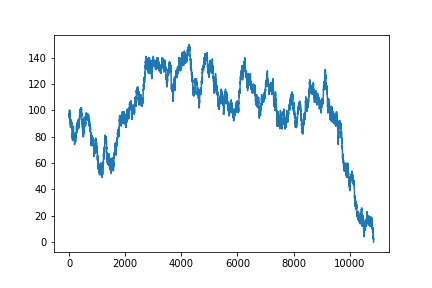
\includegraphics[width = .5\textwidth]{gamblers_ruin.png}
\end{center}